\section{NeST-Com Framework}
\subsection{System Model and Next-Scale Representation}
\begin{figure*}[t]
\centering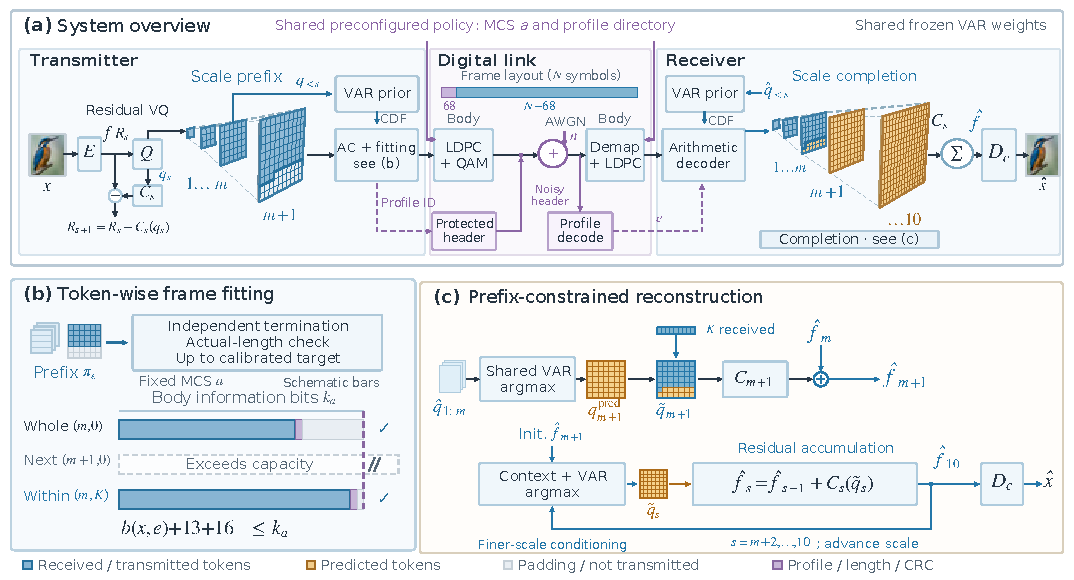
\includegraphics[width=\textwidth]{figure1_final.pdf}
\caption{NeST-Com. (a) The shared policy fixes the MCS and profile directory; the protected Profile ID selects the endpoint. VAR and known coarse tokens provide coding probabilities. (b) Independently terminated prefix bitstreams up to the target endpoint fit the body capacity; bars are schematic. (c) Received tokens overwrite boundary predictions. Recursive state updates accumulate residuals and condition each finer scale before decoding. Unreceived boundary positions retain their coarse-conditioned predictions.}
\label{fig:system}
\end{figure*}
Fig.~\ref{fig:system} illustrates the NeST-Com framework. We transmit $x\in[0,1]^{256\times256\times3}$ using $N$ complex symbols over AWGN,
\begin{equation}
y=s+n,\quad n\sim\mathcal{CN}(0,\sigma^2 I_N),\quad
\mathrm{SNR}=10\log_{10}(E_s/\sigma^2),
\label{eq:channel}
\end{equation}
with nominal symbol energy $E_s=2$ without per-frame renormalization. TX applies the frozen policy calibrated for its design SNR, whereas RX uses the actual noise variance for log-likelihood ratios (LLRs). A terminated rate-$1/2$ convolutional code protects the 12-bit profile ID and CRC16 in a fixed 68-symbol header, while the remaining $N-68$ symbols carry the LDPC-coded body with public frame-dependent scrambling.

The frozen VAR tokenizer produces ten residual token maps $q_s$, with side lengths $(1,2,3,4,5,\allowbreak 6,8,10,13,16)$ and a 4096-entry codebook~\cite{var}. Let $L_s$ denote the number of positions at scale $s$, and let $C_s$ denote codebook lookup followed by upsampling to the full latent grid and the scale-dependent residual transform. The latent sum $\sum_s C_s(q_s)$ progressively refines a full-field description, and the decoder $\Dc$ is fine-tuned once and frozen (Supplement~S1). Because token probabilities at each scale depend only on complete coarser maps, RX can reproduce the transmitter's integer cumulative distribution functions (CDFs, total frequency $2^{24}$) and decode any independently terminated prefix.

\subsection{Within-Scale Endpoints and the Nondecreasing-Length Rule}
An endpoint $e=(m,K)$ retains complete coarse maps and a raster-ordered boundary prefix:
\begin{equation}
\pi_e=(q_1,\ldots,q_m,q_{m+1,1:K}).
\label{eq:prefix}
\end{equation}
For $K=0$, including $e=(10,0)$, the boundary prefix is empty, and raster order specifies positions without a mask. WHOLE permits $(m,0)$ for $m=4,\ldots,10$. NeST permits every integer $K=0,\ldots,L_{m+1}-1$ for $m=4,\ldots,9$, plus $(10,0)$, yielding 651 endpoints from 30 to 680 tokens. Quarter and Eighth retain $K=\lfloor jL_{m+1}/d\rfloor$ ($j=1,\ldots,d-1$, $d=4,8$) plus complete-scale boundaries without duplicates; Token is the default grid.

For MCS $a=(M,r)$, the coded body carries $n_a=(N-68)\log_2M$ coded bits and $k_a=\lfloor rn_a\rfloor$ information bits. Let $b(x,e)$ be the actual bit length of the independently terminated arithmetic code for prefix $\pi_e$. Feasibility requires
\begin{equation}
b(x,e)+29\leq k_a,
\label{eq:budget}
\end{equation}
giving source-bit capacity utilization $\eta(x,e)=b(x,e)/(k_a-29)$, after reserving a 13-bit payload length and CRC16. Unused bits are zero-padded before 5G NR LDPC coding, rate matching~\cite{nr}, and QAM.

A public method/MCS directory, frozen before calibration and shared across images, maps source profiles to endpoints and includes a NULL profile. One traversal shares scale-wise probability evaluation and incremental coding, while non-mutating termination yields independent prefix bitstreams rather than slices of a longer codeword.

The fitting rule rests on a coder-specific property: under our fixed token/CDF traversal and 32-bit non-mutating finalization, the terminated length after $t$ tokens is $b_t=E_t+P_t+2$, where $E_t$ and $P_t$ count emitted and pending-underflow bits. Every renormalization increments $E_t+P_t$ by one and other interval updates preserve it; hence $b_t$ is nondecreasing, and feasible endpoints under any fixed MCS and ceiling form an initial segment. TX thus selects the longest feasible token prefix by a single incremental scan; if no source prefix fits, it sends a NULL frame with a two-bit zero payload over the full $N$-symbol budget.

\ifCLASSOPTIONonecolumn\else\begin{figure*}[t]
\centering
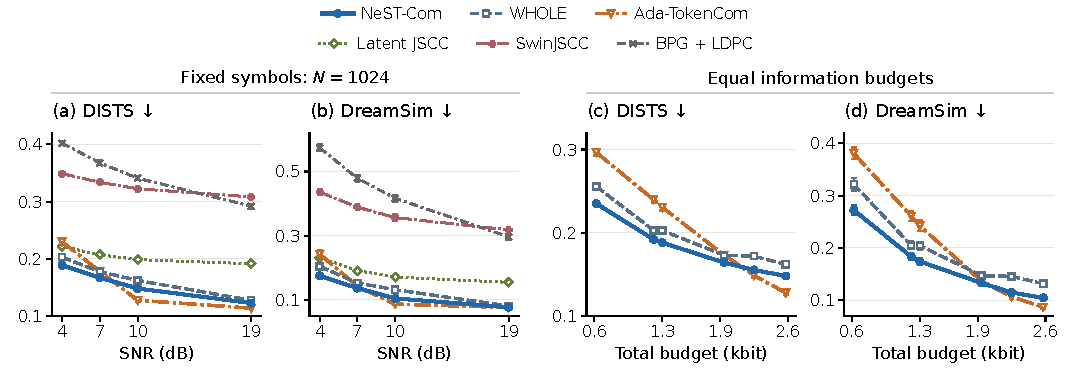
\includegraphics[width=\linewidth]{figure2_1x4.pdf}
\caption{Source-referenced reconstruction on 500 ImageNet images. (a,b) Six methods at $N=1024$; WHOLE, NeST and Ada share the 12-MCS calibration procedure. Three outcomes per source include gray failures. (c,d) Equal, error-free information budgets pay 57 shared protocol bits and Ada's additional 10-bit class; WHOLE/NeST share ceiling $(10,0)$. Points and bars are equal-source means and pointwise 95\% source-bootstrap intervals after within-source averaging. Ada-TokenCom is the predicted-class, fixed-frame adaptation. Lower values are favorable.}
\label{fig:performance}
\end{figure*}
\fi
\subsection{Prefix-Constrained Reconstruction}
Any invalid profile CRC or catalogue entry, body CRC, declared length, padding, or arithmetic stream---as well as any valid NULL frame---outputs fixed gray (RGB $0.5$) and remains in all metric denominators. Otherwise, RX decodes the prefix via the shared CDFs. At $e=(10,0)$, all maps are decoded directly; for an incomplete prefix, RX predicts the boundary map by coarse-conditioned argmax and overwrites the $K$ received positions:
\begin{equation}
\tilde q_{m+1,i}=\begin{cases}\hat q_{m+1,i},&i\leq K,\\q^{\mathrm{pred}}_{m+1,i},&i>K.\end{cases}
\label{eq:overwrite}
\end{equation}
RX then recursively generates finer maps and decodes the image:
\begin{equation}
\hat x=\Dc\!\left(\sum_{s=1}^{10}C_s(\tilde q_s)\right).
\label{eq:reconstruction}
\end{equation}
Recovered boundary tokens both correct the boundary scale's residual contribution and, via the merged map $\tilde q_{m+1}$, condition finer-scale predictions without a same-scale loop (at the final scale, overwrite modifies only the residual). Supplement~S1 details the full algorithm, proof, and numerical protocol.
